\documentclass[border=5pt]{article}
% ------- TikZ Preamble -------
\usepackage{tikz}
\usetikzlibrary{knots,hobby,calc,intersections,decorations.pathreplacing,decorations.markings,shapes.geometric,spath3}
\tikzset{ knot diagram/every strand/.append style={ultra thick, black}}

\newif\ifsstguides
\sstguidestrue

\newcommand{\SSTGuidesPoints}[2]{% #1=basename (e.g. P), #2=last index
  \ifsstguides
    \foreach \i in {1,...,#2}{
      \fill[blue] (#1\i) circle (1.2pt);
      \node[blue,font=\scriptsize,above] at (#1\i) {\i};
    }
    \draw[gray!40, dashed]
    \foreach \i [remember=\i as \lasti (initially 1)] in {2,...,#2,1} { (#1\lasti)--(#1\i) };
  \fi
}
% ------- TikZ Preamble -------



\begin{document}


    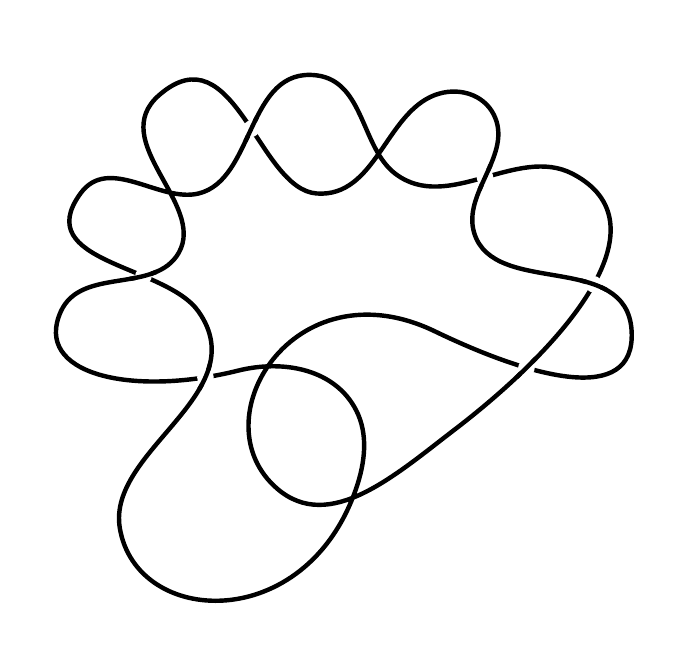
\begin{tikzpicture}[use Hobby shortcut]
    \coordinate (P1) at (0.50, -2.75);
    \coordinate (P2) at (-2.50, -3.25);
    \coordinate (P3) at (-1.50, -0.50);
    \coordinate (P4) at (-3, 1);
    \coordinate (P5) at (-1.50, 1);
    \coordinate (P6) at (0, 2.50);
    \coordinate (P7) at (1, 1.25);
    \coordinate (P8) at (3.25, 1.25);
    \coordinate (P9) at (1.75, -2);
    \coordinate (P10) at (-0.50, -2.75);
    \coordinate (P11) at (1.50, -0.75);
    \coordinate (P12) at (4, -0.75);
    \coordinate (P13) at (2, 0.50);
    \coordinate (P14) at (2.25, 2);
    \coordinate (P15) at (1.50, 2.25);
    \coordinate (P16) at (0, 1);
    \coordinate (P17) at (-2, 2.25);
    \coordinate (P18) at (-1.75, 0.25);
    \coordinate (P19) at (-3.25, -0.50);
    \coordinate (P20) at (-1, -1.25);
    \coordinate (P21) at (0.50, -1.75);% = P1

    \begin{knot}[
        consider self intersections,
        clip width=5pt, clip radius=3pt,
        ignore endpoint intersections=true,
        flip crossing/.list={2,4,6,8,10,12,14,16,18},
        % draft mode=crossings,
    ]
    \strand
    ([closed] P1)..(P2)..(P3)..(P4)..(P5)..(P6)..(P7)..(P8)..(P9)..(P10)..(P11)..(P12)..(P13)..(P14)..(P15)..(P16)..(P17)..(P18)..(P19)..(P20)..(P21);
    \end{knot}
    \SSTGuidesPoints{P}{21}
    \end{tikzpicture}



\end{document}